\documentclass[12pt,a4paper]{article}
\usepackage{fullpage}
\usepackage[top=2cm, bottom=4.5cm, left=2.5cm, right=2.5cm]{geometry}
\usepackage{amsmath,amsthm,amsfonts,amssymb,amscd}
\usepackage{lastpage}
\usepackage{enumitem}
\usepackage{fancyhdr}
\usepackage{mathrsfs}
\usepackage{xcolor}
\usepackage{graphicx}
\usepackage{listings}
\usepackage{hyperref}
\usepackage{tikz}
\usetikzlibrary{shapes,backgrounds}
\usepackage[utf8]{inputenc}
\usepackage[ruled, vlined]{algorithm2e}
% \usepackage{apacite}
\usepackage{csquotes}

% Edit these as appropriate
\newcommand\course{Reinforcement Learning}
\newcommand\NetID{sliu1@uvm.edu}
\newcommand\Author{Sida Liu}
\pagestyle{fancyplain}
\headheight 35pt
\lhead{\NetID\\\Author}
% \chead{\textbf{\Large Assignment \chapternumber }}
\rhead{\course \\ \today}
\lfoot{}
\cfoot{}
\rfoot{\small\thepage}
\headsep 1.5em

\setlength{\parskip}{\baselineskip}%
\setlength{\parindent}{0pt}%

\newenvironment{list_abc}
{ \begin{enumerate}[label=(\alph*)] }
{ \end{enumerate} }

\newenvironment{list_iv}
{ \begin{enumerate}[label=\roman*.] }
{ \end{enumerate} }

\hypersetup{
    colorlinks=true,
    linkcolor=blue,
    filecolor=magenta,      
    urlcolor=cyan,
}

\usepackage{tcolorbox}
\usepackage{booktabs}


\begin{document}

\section{Revised Project Proposal}

\subsection{Response}
\begin{tcolorbox}
    Neat project proposal! It sounds like the tracer bullet version is one where you:

    Code up an RNN to produce high level abstractions, which are functions of the current state.
    
    Learn a policy over these high level states.
\end{tcolorbox}
Does ``tracer bullet'' mean proof-of-concept? I googled this phrase but I am still not quite sure. :D Sorry about my English.

And Yes, RNN will be a key component in this architecture.

\begin{tcolorbox}
    Will this high level policy interact with the lower-level policy over observations?
\end{tcolorbox}
In Section \ref{section:multi-rl-or-multi-rnn}, I will compare multi-RL and multi-RNN. I will come to the conclusion that multi-RNN can be equivalent to multi-RL, and multi-RNN has a major advantage: the gradient is available.
So I'll use multi-RNN. (But I am not quite sure so many papers are using hierarchical-RL, maybe I am wrong?)

\begin{tcolorbox}
    Do you intend to learn over a family of possible high level policies?
\end{tcolorbox}
I'll gradually increase the complexity of the model and produce different higher representations.
There will be only one RL policy at the top to consume all the representations.

\begin{tcolorbox}
    I am particularly interested in whether/how you might forsee using such a model for the embodied agent problem you've talked about.
\end{tcolorbox}
I might use Multi-Robot Continuous Control task as one of the testbed (control different robots to move forward).
But the model developed in this work should be a general RL model that can work beyond robotics.

\subsection{Structure}
The deliverable will be a piece of open-source software.

\subsection{Topic}

\subsubsection{Motivation}
In 2017, Yoshua Bengio submitted an arXiv article named \emph{The Consciousness Prior} \cite{bengio_consciousness_2019}. 
He proposed the \emph{Consciousness Prior Theory}, which is about how, in his opinion, the \emph{Consciousness} works and how to implement the \emph{Global Workspace Theory} using recently developed \emph{Deep Learning} technology.
There are two major parts in his theory, the \emph{Consciousness} $c$ and the \emph{Unconsciousness} $h$.

In Bengio's paper, he thinks the high-level abstraction (a.k.a. the \emph{Unconsciousness}) $h$ is produced by some representation RNN function $F$, so that

\begin{equation*}
    h_t = F(x_t, h_{t-1})
\end{equation*}

where $x_t$ is the \emph{observation} at time $t$, and $h_{t}$ is the \emph{unconscious representation state} (or \emph{high-level state}) at time $t$.

I will focus on the $h$ in this course project because it is more practical and is the foundation before we get anything similar to the \emph{Consciousness}.

\subsubsection{Big Picture of Deep Reinforcement Learning}
Our objective is to get a good $h$, but how can we get it.

Deep Learning is trying to do hierarchical information abstraction since its invention. 
CNN, RNN, Attention model, and many other Deep Learning models are very good tools to do this job.

In the setting of Reinforcement Learning, we can simply situate the agent in an environment, and use a high-level reward function to specify the goal.

At each time step, we can pass observation through the neural network model of the agent and get a value of that state (or action);
we can also use the Temporal Difference (TD) method to get a value of that state (or action).
We assume the TD method gives us the right value, so we adjust the parameters of the neural network model of the agent to make two values consistent.
This consistency is what we usually use to train an agent in Deep Reinforcement Learning.

\subsubsection{Additional training signal beside TD method}
What if the TD method doesn't give us the perfect value function? Do we have other sources of learning signals?

One possible learning signal can come from temporal consistency.
For example, we have two observations of two consecutive time steps.
We can assume the world doesn't change much in one single step, so the meaning of those two observations should be similar.
So we can pass two observations through the neural network model and compare two values produced.
They should be consistent.
And we can train the neural network model based on this consistency.

This might be an additional source for learning besides the TD method. 
I mention this because I think this is interesting, but it might not be implemented in this work.

\subsubsection{Course Project Plan: Step 0}

I'll start the project with an empty framework without any RNNs illustrated in Fig \ref{fig:starting_point}.

\begin{figure}[h]
    \centering
    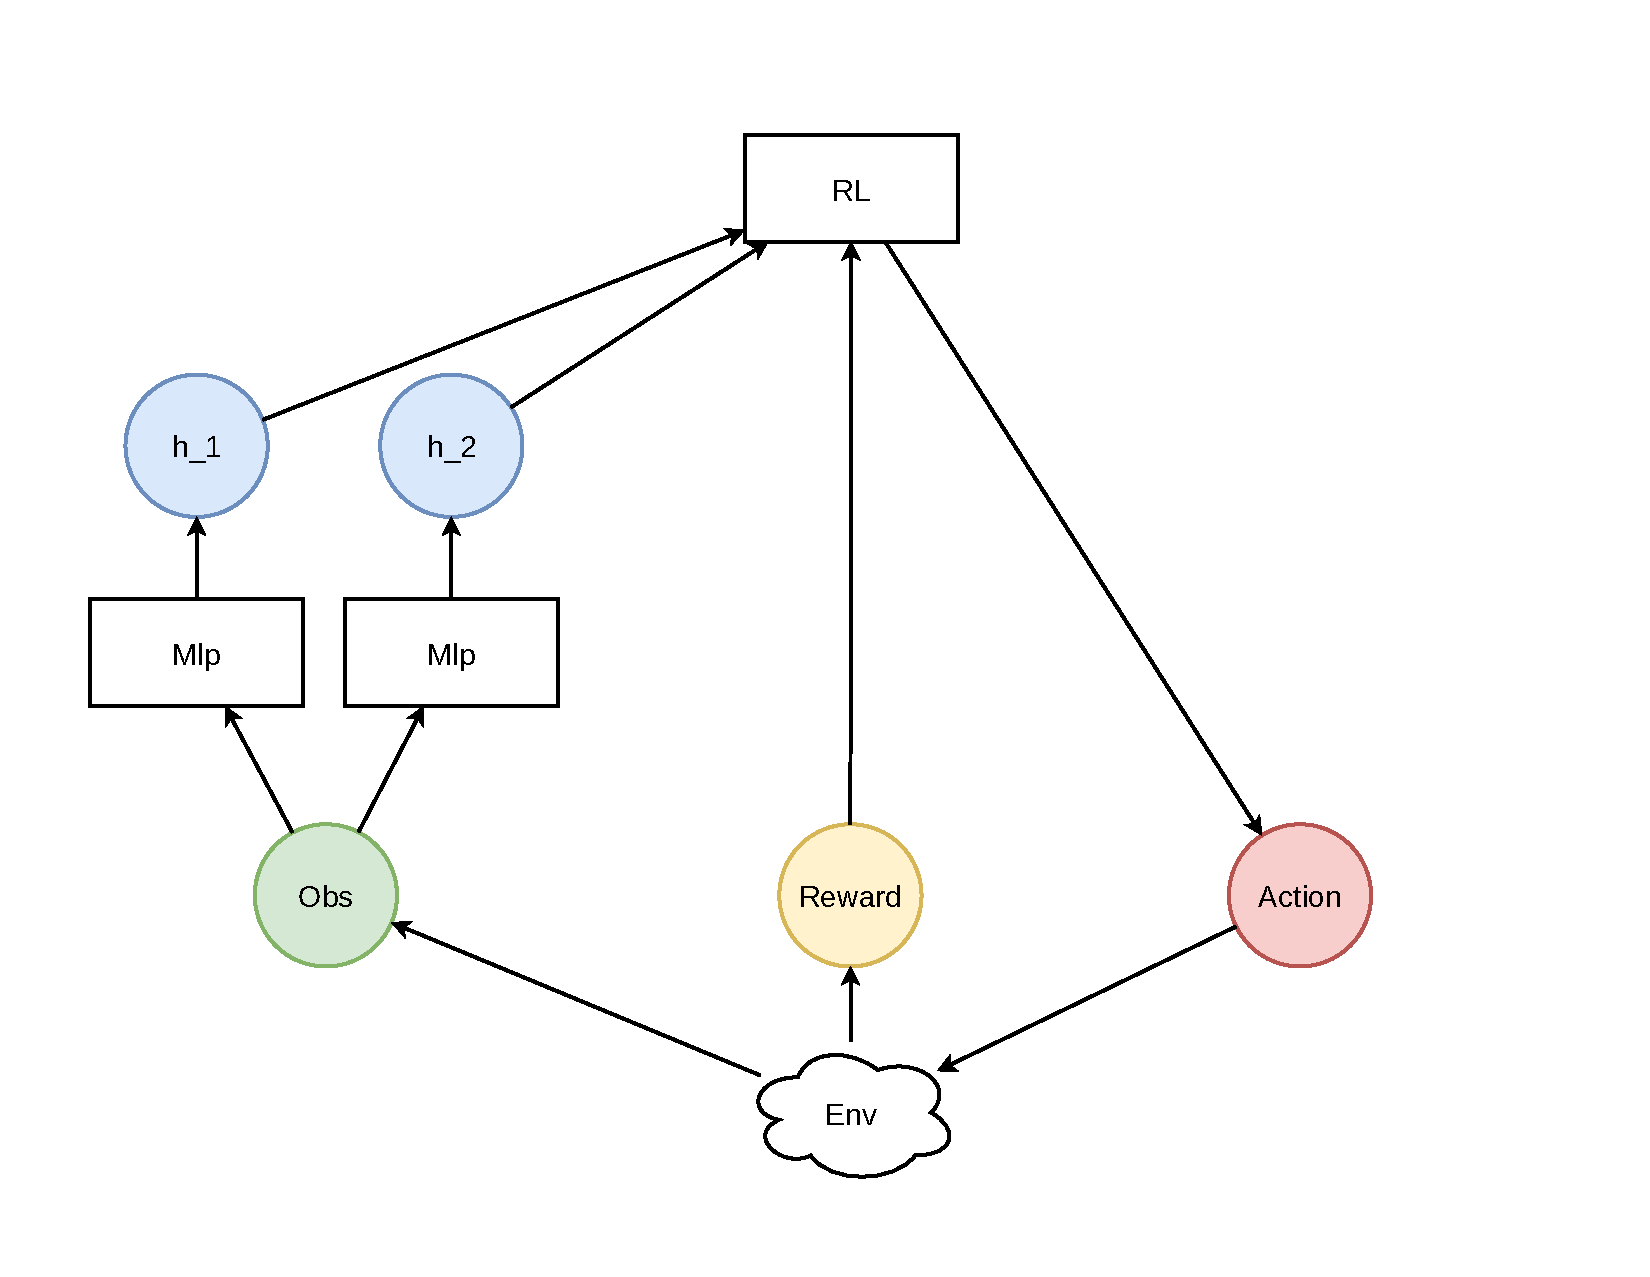
\includegraphics[width=0.8\textwidth]{images/step-0.pdf}
    \caption{Starting point: without any RNN}
    \label{fig:starting_point}
\end{figure}

This is a standard RL model with two different MultiLayer Perceptron (MLP) modules.
The representation (in blue) will be concatenated and pass into the RL core algorithm.

Later in this project, my job is to produce more and better representations $h$'s for the RL core algorithm on the left side.
I'll introduce RNNs and other tools available in Deep Learning.

Once we have more than enough $h$'s, and if there is time left,  we can introduce attention mechanism to filter them before passing into the RL.

I am not very sure about the right side of the diagram yet.
For example, in conventional hierarchical RL, people use options to execute a sequence of actions, but I am not sure if it is necessary in this framework.
Maybe in this project, I'll just leave it as simple as it is.

\subsubsection{Testing Environments}
My algorithm should be general, so it can work in different environments.

One possible testbed is the Continuous Control problem.
For example, locomotion is my most familiar task.

I also wish to test it in some multi-player games, so maybe I can ask my agent to play with someone else's agent.

\subsection{World Model: An Example}
David Ha et al. 2018 proposed the World Model \cite{ha_world_2018}.
As illustrated in Fig \ref{fig:world_model}, it utilizes a VAE and an RNN to make a model so that the agent can not just see the compressed current observation but can also predict the future.
Both current observation and the prediction of the future are passed into an RL agent.

Interestingly, the RNN takes in the action and $h_1$ from previous time step. I understand the action of current step is not available, but why the previous $h_1$?

Also, the inputting of previous action indicates that the reward could also be an input. hmm... My interpretation is that, since we are facing a POMDP, the observation doesn't capture all the information, for example, the previous action. So I'll treat previous action and previous reward as additional observations.

Overall, this model is a good demonstration of the framework we constructed here.

However, the paper only has one VAE and one RNN, so it's not possible to capture features at different scales.
As illustrated in Fig \ref{fig:starting_point}, I prefer multiple modules that can extract representations at multiple scales.

\begin{figure}[h]
    \centering
    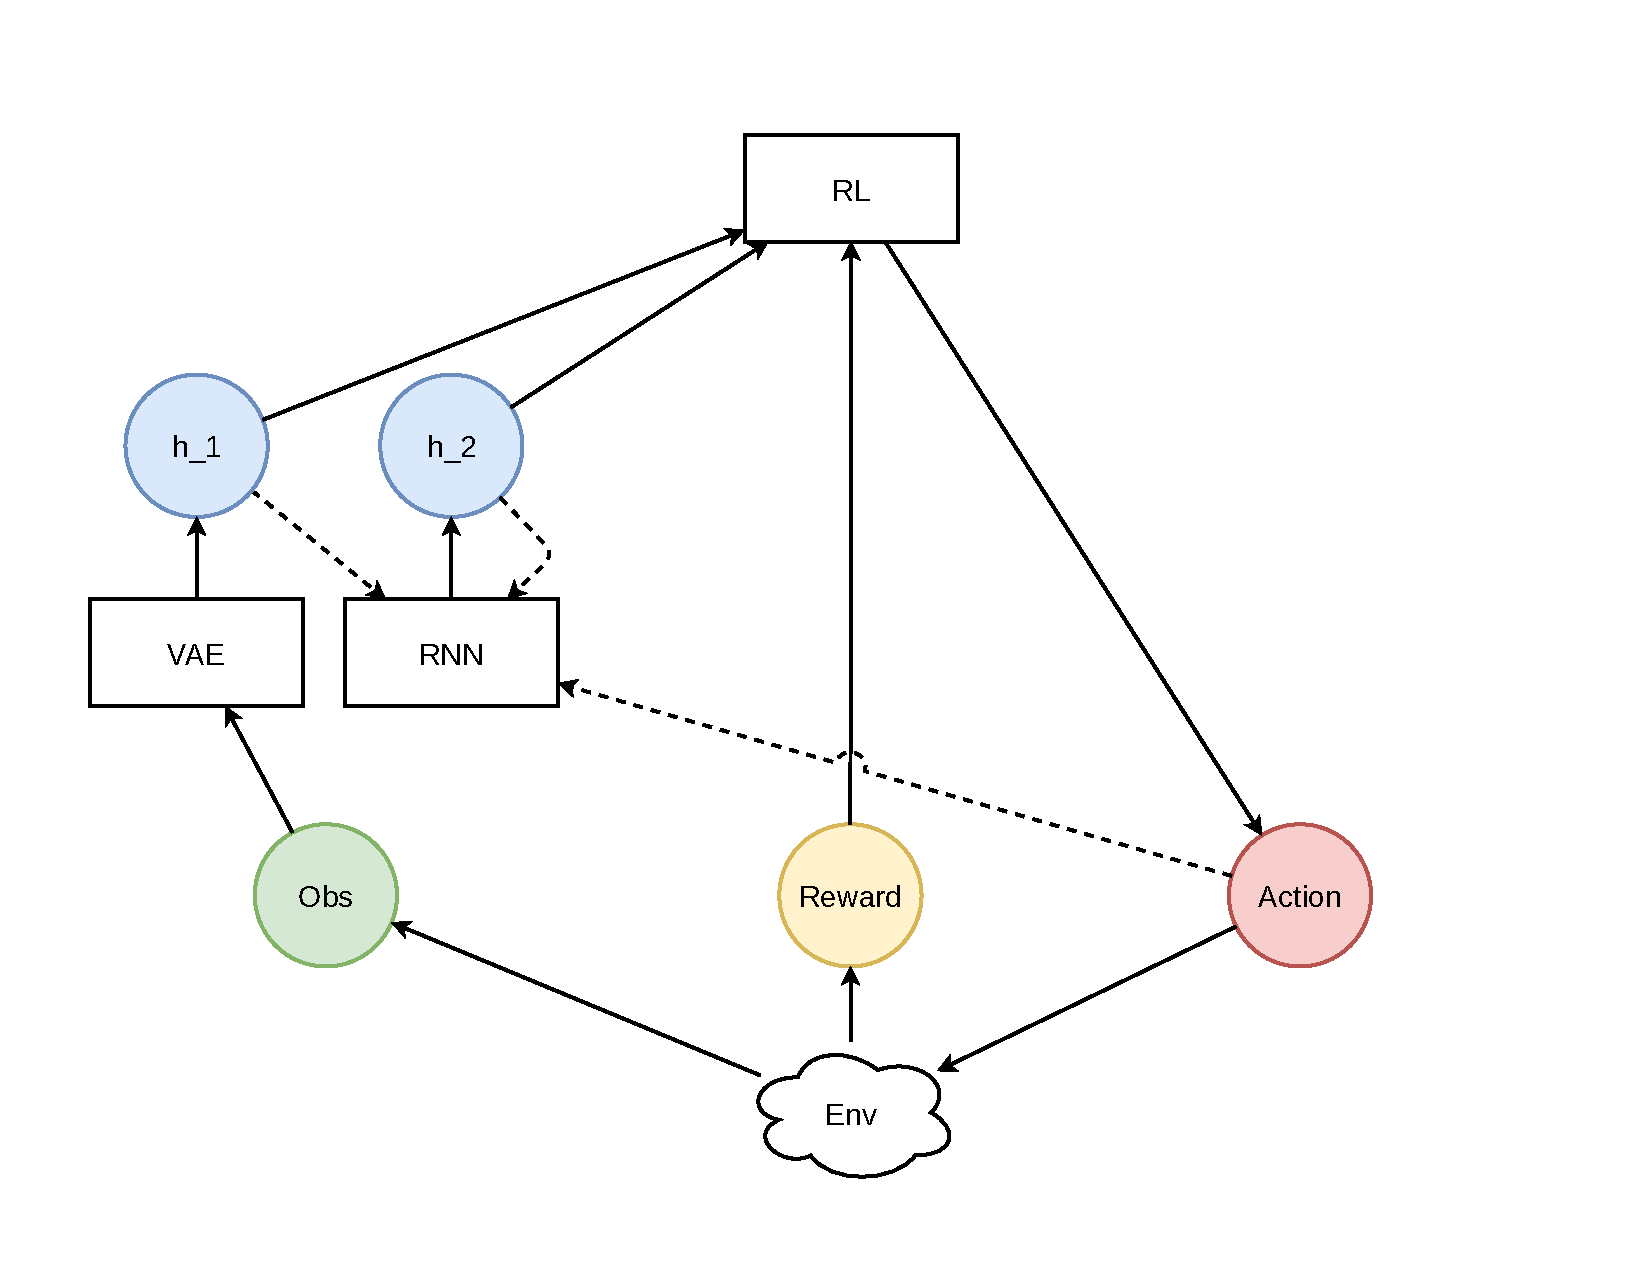
\includegraphics[width=0.8\textwidth]{images/world-model.pdf}
    \caption{The World Model, re-illustrated to fit in our framework. Dashed line stands for the information is from the previous time step.}
    \label{fig:world_model}
\end{figure}

\subsection{Multiple RLs or Multiple RNNs?} \label{section:multi-rl-or-multi-rnn}
Before I read these two papers \cite{li2017learning}\cite{andrychowicz2016learning}, I thought RL and RNN are simply different creatures.
And then, I looked at these two approaches of making learned optimizers to replace hand-designed optimizer such as Adam, and I realized there are so many similarities.

One views the optimizer as an RL agent\cite{li2017learning}, and the other views the optimizer as an RNN network\cite{andrychowicz2016learning}.
Here is a brief comparison:

\subsubsection{RL: Learning to Optimize}
% 
Li et al. proposed this idea in 2016 \cite{li2016learning}, which is very similar to my idea.
In Li et al., 2016, the observation contains: (1) Current parameters, $\theta$, (2) The $\Delta \mathcal{L}$ in recent $H$ time steps, (3) The $\nabla_{\theta} \mathcal{L}$ in recent $H$ time steps. (I changed the notation to be aligned with this document.)
The action contains: (1) the update steps, $\Delta \theta = \alpha \nabla_{\theta} \mathcal{L}$.
The goal is to minimize the total area under the learning curve at meta-test time.
The reward function (cost function) is the negative value of outer loss function, $- \mathcal{L}$.
They chose Guided Policy Search (GPS) as the RL algorithm for the optimizer.

\begin{figure}[h]
    \centering
    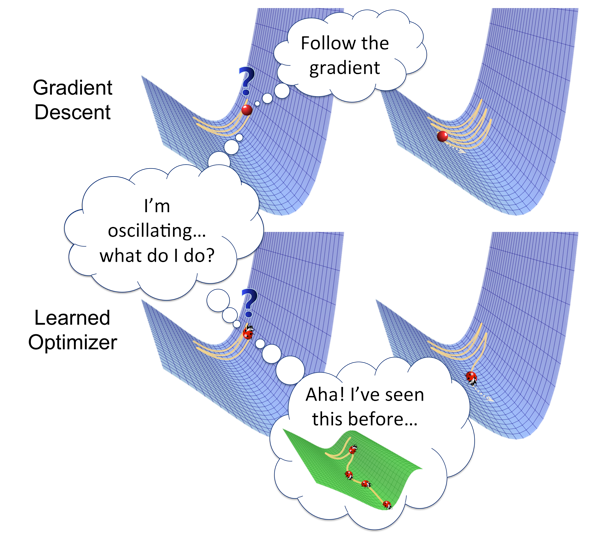
\includegraphics[width=0.5\textwidth]{images/learn-to-optimize.png}
    \caption{Illustration of the Paper \emph{Learning to Optimize}. Source: \href{https://bair.berkeley.edu/blog/2017/09/12/learning-to-optimize-with-rl/}{Blog}}
    \label{fig:world_model}
\end{figure}

Li et al. 2017 provide more details on implementation \cite{li2017learning}, though source code is not available.
The learned optimizer was then tested on several image datasets, which outperforms Adam, AdaGrad, RMSprop in the experiments.

In general, I think Li's implementation can be improved somehow. 
At least I should be able to produce a reusable package that can be easily used in PyTorch.

\subsubsection{RNN: Learning to learn by gradient descent by gradient descent}
In contrast, Andrychowicz et al. 2016\cite{andrychowicz2016learning} formulate the optimizer as an RNN neural network.
At every time step, the current parameters $\theta$, and the gradients $\nabla_\theta \mathcal{L}$ are the input to the RNN, along with the hidden state $hidden_{t-1}$ (to avoid using the notation $h$ here) of the last step.
Just like the RL model, the RNN also produces the update steps, $\Delta \theta$, and the outer network applies the update steps.
Critically, because the whole model is differentiable, so they can directly compute gradients for the RNN optimizer from that step.

Also, to reduce the requirement of memory and make the model more flexible, the RNN model doesn't take concatenated parameters and gradients but take one parameter and one gradient at a time, so all parameters from outer networks pass through the RNN model, producing multiple hidden states and the update steps for their corresponding parameters, respectively.

\subsubsection{My Lesson}
I am not planning to use learned optimizers in my course project.
I'll still use Adam.
However, from this comparison, the takeaway for me is that, in my hierarchical networks, there will be no need to construct multiple RL agents.
We should not formulate problems as an RL problem if the gradients are directly available.

\bibliographystyle{unsrt}
\bibliography{reference.bib}


\end{document}
